\documentclass[cs4size,a4paper]{ctexart}   
%==================== 数学符号公式 ============
\usepackage{amsmath}                 % AMS LaTeX宏包
\usepackage[style=1]{mdframed}
\usepackage{amsthm}
\usepackage{amsfonts}
\usepackage{mathrsfs}                % 英文花体字 体
\usepackage{bm}                      % 数学公式中的黑斜体
\usepackage{bbding,manfnt}           % 一些图标,如 \dbend
\usepackage{lettrine}                % 首字下沉,命令\lettrine
\def\attention{\lettrine[lines=2,lraise=0,nindent=0em]{\large\textdbend\hspace{1mm}}{}}
\usepackage{longtable}
\usepackage[toc,page]{appendix}
\usepackage{geometry}                % 页边距调整
\geometry{top=3.0cm,bottom=2.7cm,left=2.5cm,right=2.5cm}
%====================公式按章编号==========================
\numberwithin{equation}{section}
\numberwithin{table}{section}
\numberwithin{figure}{section}
%================= 基本格式预置 ===========================
\usepackage{fancyhdr}
\pagestyle{fancy}
\fancyhf{}  
\fancyhead[C]{\zihao{5}  \kaishu python编程语言课程作业:社交媒体数据爬取分析}
\fancyfoot[C]{~\zihao{5} \thepage~}
\renewcommand{\headrulewidth}{0.65pt} 
\CTEXsetup[format={\centering\bfseries\zihao{-2}},name={第, 章}]{section}
\CTEXsetup[nameformat={\bfseries\zihao{3}}]{subsection}
\CTEXsetup[nameformat={\bfseries\zihao{4}}]{subsubsection}
%================== 图形支持宏包 =========================
\usepackage{subfigure}
\usepackage{graphicx}                % 嵌入png图像
\usepackage{color,xcolor}            % 支持彩色文本、底色、文本框等
\usepackage{hyperref}                % 交叉引用
\usepackage{caption}
\captionsetup{figurewithin=section}
%==================== 源码和流程图 =====================
\usepackage{listings}                % 粘贴源代码
\usepackage{xcolor}
\usepackage{color}
\definecolor{dkgreen}{rgb}{0,0.6,0}
\definecolor{gray}{rgb}{0.5,0.5,0.5}
\definecolor{mauve}{rgb}{0.58,0,0.82}
 \usepackage{xcolor}
 \lstset{
  %行号
    numbers=left,
    %背景框
    framexleftmargin=8mm,
    frame=none,
     %背景色
    %backgroundcolor=\color[rgb]{1,1,0.76},
     backgroundcolor=\color[RGB]{245,245,244},
     %样式
   keywordstyle=\bf\color{blue},
   identifierstyle=\bf,
    numberstyle=\color[RGB]{0,192,192},
    commentstyle=\it\color[RGB]{0,96,96},
   stringstyle=\rmfamily\slshape\color[RGB]{128,0,0},
   %显示空格
    showstringspaces=false
 }


%--------------------
\hypersetup{hidelinks}
\usepackage{booktabs}  
\usepackage{shorttoc}
\usepackage{tabu,tikz}
\usepackage{float}

\usepackage{multirow}



\tabcolsep=1ex
\tabulinesep=\tabcolsep
\newlength\tikzboxwidth
\newlength\tikzboxheight
\newcommand\tikzbox[1]{%
        \settowidth\tikzboxwidth{#1}%
        \settoheight\tikzboxheight{#1}%
        \begin{tikzpicture}
        \path[use as bounding box]
                (-0.5\tikzboxwidth,-0.5\tikzboxheight)rectangle
                (0.5\tikzboxwidth,0.5\tikzboxheight);
        \node[inner sep=\tabcolsep+0.5\arrayrulewidth,line width=0.5mm,draw=black]
                at(0,0){#1};
        \end{tikzpicture}%
        }

\makeatletter
\def\hlinew#1{%
  \noalign{\ifnum0=`}\fi\hrule \@height #1 \futurelet
   \reserved@a\@xhline}
   
\newcommand{\tabincell}[2]{\begin{tabular}{@{}#1@{}}#2\end{tabular}}%

\usepackage{subfigure}

\usepackage{CJK}
\usepackage{ifthen}

\usepackage{graphicx} 
\newcommand{\HRule}{\rule{\linewidth}{0.5mm}}

\newtheorem{Theorem}{定理}
\newtheorem{Lemma}{引理} 
%%使得公式随章节自动编号
\makeatletter
\@addtoreset{equation}{section}
\makeatother
\renewcommand{\theequation}{\arabic{section}.\arabic{equation}}

%-------------------------
	
\usepackage{pythonhighlight}
\usepackage{tikz}                    
\usepackage{tikz-3dplot}
\usetikzlibrary{shapes,arrows,positioning}
%===================   正文开始    ===================
\begin{document}
\bibliographystyle{gbt7714-2005}     %论文引用格式
%===================  定理类环境定义 ===================
\newtheorem{example}{例}              % 整体编号
\newtheorem{algorithm}{算法}
\newtheorem{theorem}{定理}            % 按 section 编号
\newtheorem{definition}{定义}
\newtheorem{axiom}{公理}
\newtheorem{property}{性质}
\newtheorem{proposition}{命题}
\newtheorem{lemma}{引理}
\newtheorem{corollary}{推论}
\newtheorem{remark}{注解}
\newtheorem{condition}{条件}
\newtheorem{conclusion}{结论}
\newtheorem{assumption}{假设}
%==================重定义 ===================

\renewcommand{\contentsname}{目录}     
\renewcommand{\abstractname}{摘要} 
\renewcommand{\refname}{参考文献}     
\renewcommand{\indexname}{索引}
\renewcommand{\figurename}{图}
\renewcommand{\tablename}{表}
\renewcommand{\appendixname}{附录}
\renewcommand{\proofname}{证明}
\renewcommand{\algorithm}{算法} 

%============== 封皮和前言 =================
\begin{titlepage}

\begin{center}


% Upper part of the page

\includegraphics[width=0.65\textwidth]{figure/logo}\\[1cm]    

\textsc{\LARGE \bf 新闻与新媒体学院}\\[1.9cm]

\textsc{\Large \bf python编程语言课程报告}\\[0.5cm]


% Title
\HRule \\[0.4cm]
{ \huge \bfseries 共青团中央微博数据分析}\\[0.4cm]

\HRule \\[1.5cm]

% Author and supervisor
\begin{minipage}{0.4\textwidth}
\begin{center} \large

\textsc{\kaishu 姓名:杨忠强\\学号:2215310366}

\end{center}
\end{minipage}

\vfill

% Bottom of the page
{\large \today}

\end{center}

\end{titlepage}


\pagestyle{plain}
\pagenumbering{Roman}
\section*{\zihao{2} \centering \bf 摘要}

\vskip0.5cm
微博作为快速便捷的社交媒体平台,在网民舆论思潮中发挥着重要的信息引导作⽤。本次作业分析微博平台共青团中央账号的发微情况。以2019年至今其所发布的所有微博作为主要研究对象,统计分析其发微规律与时间构成情况,同时利用jieba分词提取所发微博中的高频词汇,分词后通过LDA主题模型分析其所发微博的几大主题构成,最后通过pyecharts制作可视化展现相应的结果提高交互性。
\\[0.4cm]
\textbf{关键词:}  微博,共青团中央,数据分析,可视化 
\\[2cm]
\begin{figure}[H]
    \centering
    
\includegraphics[width=12cm]{figure/wordcloudweibo.png}
\end{figure} 

\addcontentsline{toc}{section}{摘要}
      
\pagestyle{empty}
\tableofcontents 
\thispagestyle{empty}
%============== 论文正文   =================
\pagestyle{fancy}
\pagenumbering{arabic}
\section{目标简介}
本报告目的是抓取社交媒体平台数据,并进行计算分析,而后对所爬取数据进行分析和可视化展示。

\subsection{数据爬取}
网络爬虫的主要目的是将互联网上的网页下载到本地形成一个或联网内容的镜像备份,通过对内容的解析之后格式化处理进行存储。本报告使用爬虫项目所用框架为scrapy。
\begin{figure}[H]
\centering
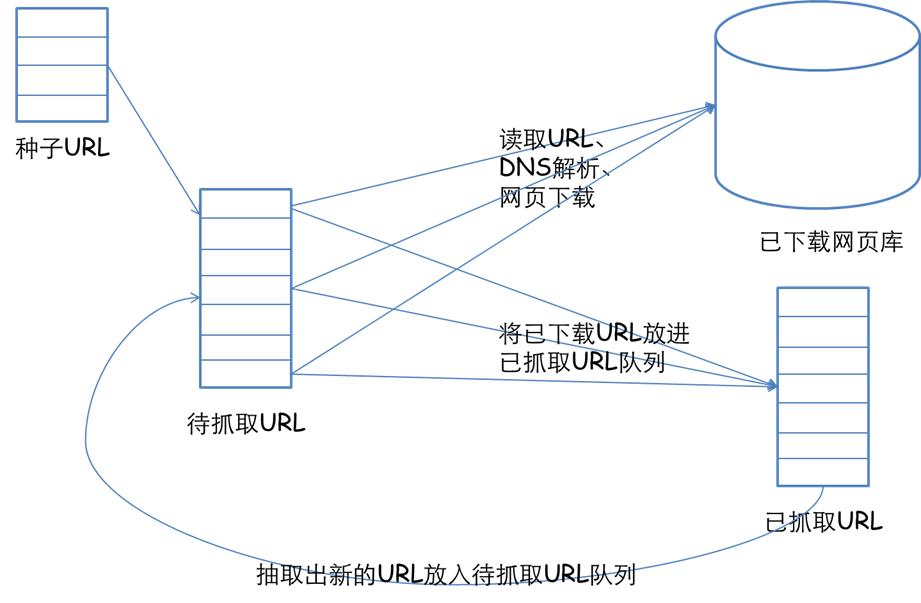
\includegraphics[width=12cm]{figure/spider.png}
\caption{爬虫示意图} \label{fig:spider}
\end{figure}

\subsection{数据分析可视化}
本报告使用pandas、jieba等库进行数据处理,具体方案将在后文阐述。可视化工具使用为pyecharts\ref{fig:pyecharts},可视化数据生成html文件后能够较好实现交互。
\begin{figure}[H]
\centering
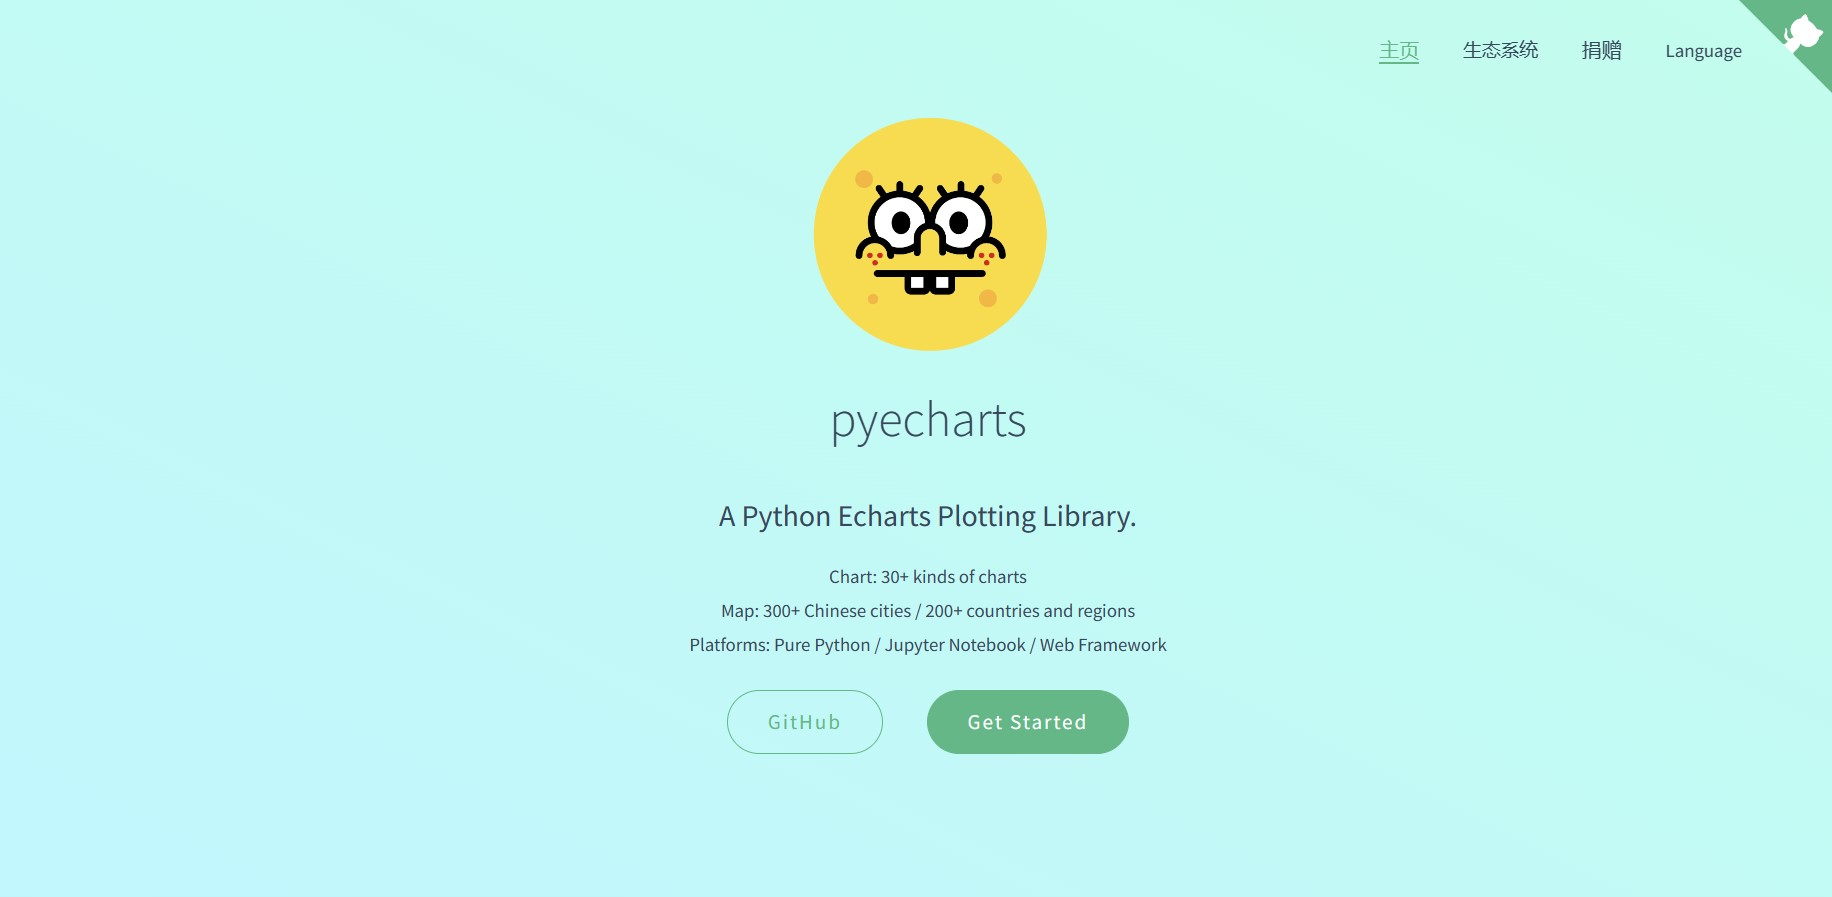
\includegraphics[width=12cm]{figure/pyecharts.jpg}
\caption{pyecharts} \label{fig:pyecharts}
\end{figure}


\subsection{运行环境}
本报告在pycharm(Community Edition 2022.2.2)的windows版本下运行,环境配置为python3.10,界面如图 \ref{fig:pycharm} 所示。
\begin{figure}[H]
\centering
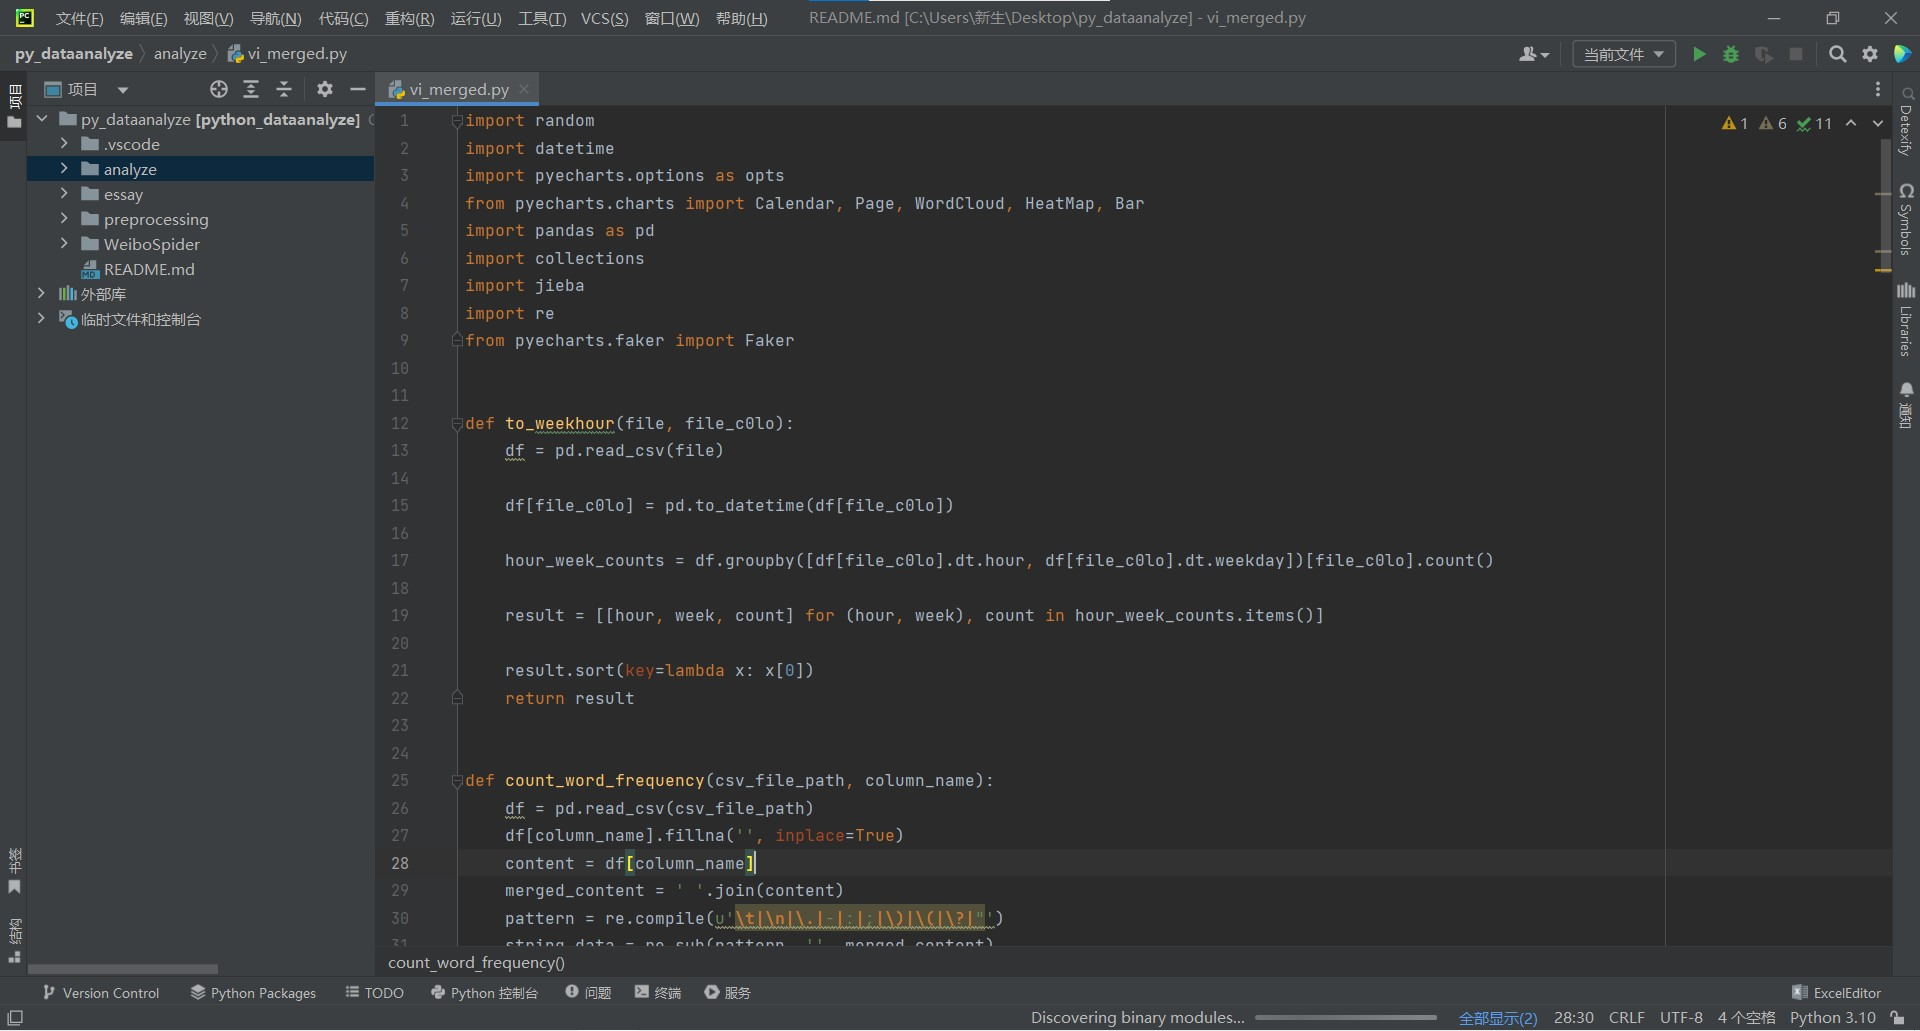
\includegraphics[width=15cm]{figure/environment_pycharm.jpg}
\caption{pycharm运行环境示意图} \label{fig:pycharm}
\end{figure}

      %
\section{数据爬取}
\subsection{爬取对象}
本报告选取共青团中央的官方微博如图 \ref{fig:gqtzy},爬取时间范围为2019年1月1日到2023年7月16日。

\begin{figure}[H]
    \centering
    
\includegraphics[width=12cm]{figure/gqtzy.jpg}
    \caption{共青团中央官方微博} \label{fig:gqtzy}
\end{figure}

\subsection{爬虫实现}
本报告数据爬取使用Github基于weibo.com的新版API构建的爬虫项目,项目地址为:https://github.com/nghuyong/WeiboSpider,项目主页如图\ref{fig:weibospider}所示。主要使用该项目下的tweet.py基于用户id进行爬虫,项目具体使用可参照其README文件。
\begin{figure}[H]
    \centering
    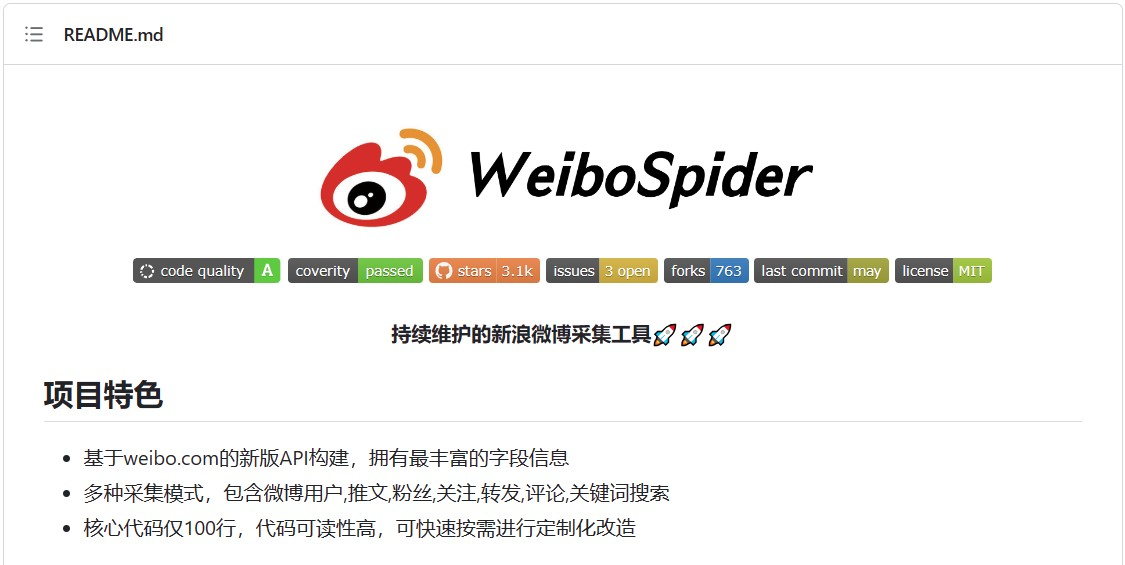
\includegraphics[width=13cm]{figure/weibospider.jpg}
    \caption{项目主页示例} \label{fig:weibospider}
\end{figure}\
该项目将爬取数据解析后存储为json格式,其单条数据示例如下所示。
\begin{python}
{
    "_id": "4762810834227120",
    "mblogid": "LqlZNhJFm",
    "created_at": "2022-04-27 10:20:54",
    "geo": null,
    "ip_location": null,
    "reposts_count": 1890,
    "comments_count": 1924,
    "attitudes_count": 12167,
    "source": "三星Galaxy S22 Ultra",
    "content": "生于乱世纵横四海,义之所在不计生死,孤勇者陈恭一生当如是。#风起陇西今日开播# #风起陇西#  今晚,恭候你!",
    "pic_urls": [],
    "pic_num": 0,
    "isLongText": false,
    "user": {
        "_id": "1087770692",
        "avatar_hd": "https://tvax1.sinaimg.cn/crop.0.0.1080.1080.1024/40d61044ly8gbhxwgy419j20u00u0goc.jpg?KID=imgbed,tva&Expires=1682768013&ssig=r1QurGoc2L",
        "nick_name": "陈坤",
        "verified": true,
        "mbrank": 7,
        "mbtype": 12,
        "verified_type": 0
    },
    "video": "http://f.video.weibocdn.com/o0/CmQEWK1ylx07VAm0nrxe01041200YDIc0E010.mp4?label=mp4_720p&template=1280x720.25.0&ori=0&ps=1CwnkDw1GXwCQx&Expires=1682760813&ssig=26udcPSXFJ&KID=unistore,video",
    "url": "https://weibo.com/1087770692/LqlZNhJFm",
    "crawl_time": 1682757213
}
\end{python}

\subsection{数据采集结果}
本报告共采集到共青团中央从2019年1月1日至2023年7月16日发微数据25244条,采集结果如图\ref{fig:outputjson}所示。
\begin{figure}[H]
    \centering
    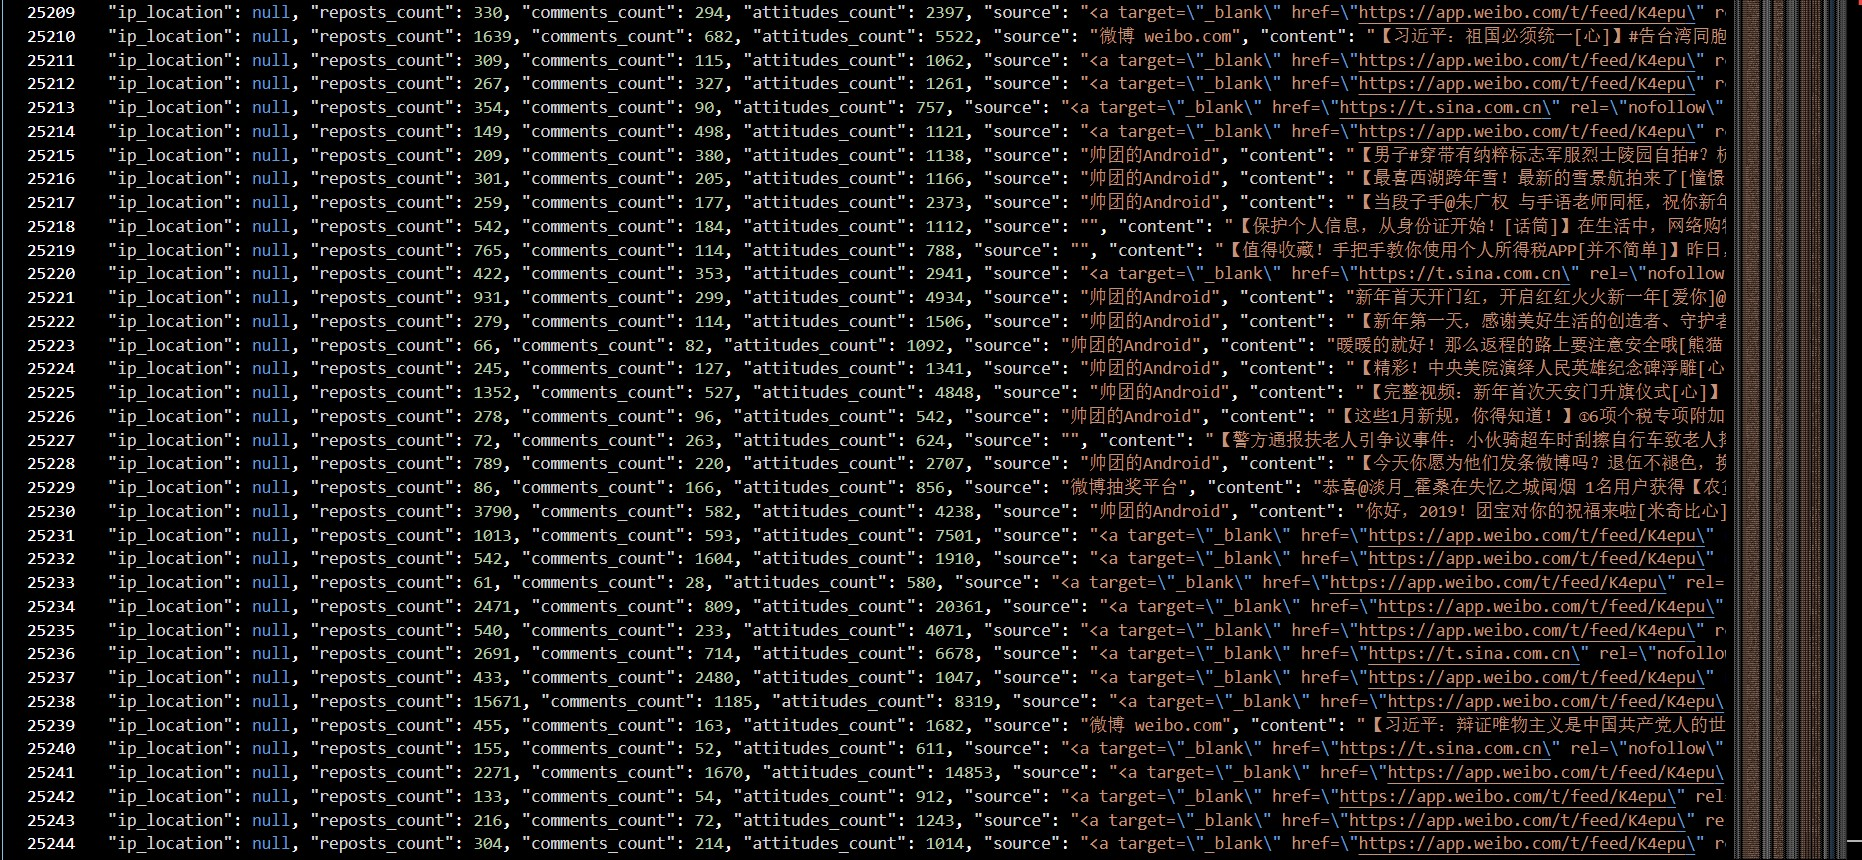
\includegraphics[width=13cm]{figure/output_1.jpg}
    \caption{数据采集结果} \label{fig:outputjson}
\end{figure}

\section{数据预处理}
与一般的数据处理全流程类似,本报告的实现过程主要包括数据的爬取、数据预处理、计算结果分析和数据的可视化展示等几个主要步骤。
\\

\subsection{数据去重与格式转换}
首先,将json文件转换为csv格式,先写入表头,后循环读取每一行的数据的key值所对应的value后输出,对应函数实现如下。
\begin{python}
def json_to_csv(input_file, output_file):
    with open(input_file, 'r', encoding='utf-8') as json_file, open(output_file, 'w', encoding='utf-8',
                                                                    newline='') as csv_file:
        writer = csv.writer(csv_file)
        writer.writerow(['user_id', 'mblogid', 'created_at', 'reposts_count', 'comments_count', 'attitudes_count',
                         'content', 'pic_urls', 'pic_num', 'isLongText', 'url', 'crawl_time'])

        for line in json_file:
            data = json.loads(line)
            user_id = data['_id']
            mblogid = data['mblogid']
            created_at = data['created_at']
            reposts_count = data['reposts_count']
            comments_count = data['comments_count']
            attitudes_count = data['attitudes_count']
            content = data['content'].replace('\n', ' ')  # 将换行符替换为空格,避免输出时自动换行
            pic_urls = data['pic_urls']
            pic_num = data['pic_num']
            islongtext = data['isLongText']
            url = data['url']
            crawl_time = data['crawl_time']

            writer.writerow([user_id, mblogid, created_at, reposts_count, comments_count, attitudes_count,
                             content, pic_urls, pic_num, islongtext, url, crawl_time])
\end{python}

此外,使用pandas的内置函数drop\_duplicates进行去重处理并使用sort\_value实现按照'created\_at'列的时间降序排列,核心代码如下。

\begin{python}
df = pd.read_csv('gqt_output.csv')
df.drop_duplicates(inplace=True)
df = df.sort_values('created_at', ascending=False)
df.to_csv('gqt_output.csv', index=False)
\end{python}

\subsection{文本内容清洗}
定义正则表达式匹配去除content中的无效文本。
\begin{python}
def clean_text(text):
    text = re.sub(r'【[^】【]+】', '', text)
    text = re.sub(r'\[[^\]\[]+\]', '', text)
    text = re.sub(r"(回复)?(//)?\s*@\S*?\s*(:|:| |$)", " ", text)  # 去除正文中的@和回复/转发中的用户名
    text = re.sub(r'\([^)(]+\)', '', text)
    text = re.sub(r'\([^)(]+\)', '', text)
    text = re.sub(r"#([^#]+)#", "", text)
    text = re.sub(r"​​​", "", text)
    text = text.replace("\n", " ")
    text = re.sub(r"↓↓", "", text)
    text = re.sub(r"(\s)+", r"\1", text)
    link_regex = r'http://t\.cn/[\w]+(,)?(?=[^\w]|,|$)'
    text = re.sub(link_regex, '', text)
    stop_terms = ['展开', '全文', '展开全文', '一个', '网页', '链接', '?【', 'ue627', 'c【', '10', '一下', '一直',
                  'u3000', '24', '12',
                  '30', '?我', '15', '11', '17', '?\\', '显示地图', '原图']
    for x in stop_terms:
        text = text.replace(x, "")
    return text.strip()
\end{python}

\section{数据分析与可视化}
\par{本报告使用可视化库为pyecharts,能够在web端实现数据交互查看,最终html文件位于ananlyze目录下,预览动态交互可运行vi\_merged.html可查看,以下部分仅展示静态图片。}

\subsection{逐年发微热力图}
统计分析每年中月日发微博频率,主要代码如下。
\begin{python}
    df = pd.read_csv('cleaned_text.csv', parse_dates=['created_at'])
    date_counts = df['created_at'].dt.date.value_counts()
    cal_result = [(date, count) for date, count in date_counts.items()]
    page = Page(page_title='共青团中央微博分析', layout=Page.DraggablePageLayout)
    for year in range(2019, 2024):
        calendar = (
            Calendar()
            .add("",
                 cal_result,
                 calendar_opts=opts.CalendarOpts(range_=str(year)),
                 daylabel_opts=opts.CalendarDayLabelOpts(name_map="cn"),
                 monthlabel_opts=opts.CalendarMonthLabelOpts(name_map="cn"),
                 )
            .set_global_opts(
                title_opts=opts.TitleOpts(title=f"{year} 年每天发微频率"),
                visualmap_opts=opts.VisualMapOpts(
                    max_=55, min_=5, orient="horizontal", is_piecewise=True, pos_top="230px", pos_left="100px",
                ),
            )
        )
\end{python}
逐年可视化热力图如下。
\begin{figure}[H]
    \centering
    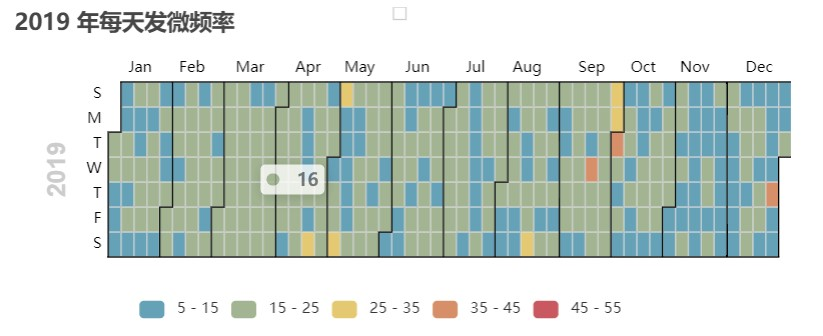
\includegraphics[width=12cm]{figure/2019.jpg}
    \caption{2019热力图} \label{fig:2019}
\end{figure}

\begin{figure}[H]
    \centering
    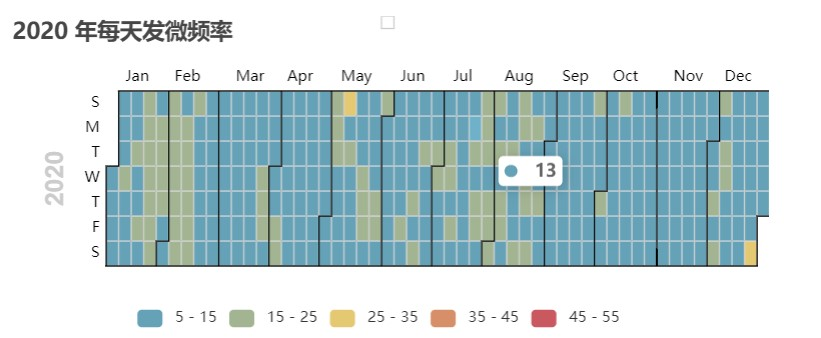
\includegraphics[width=12cm]{figure/2020.jpg}
    \caption{2020热力图} \label{fig:2020}
\end{figure}
\begin{figure}[H]
    \centering
    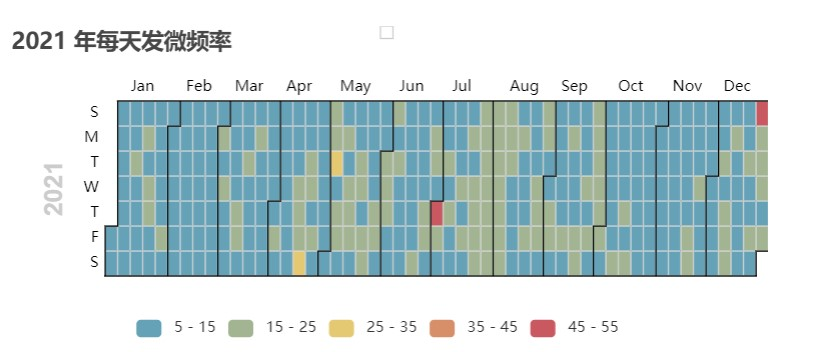
\includegraphics[width=12cm]{figure/2021.jpg}
    \caption{2021热力图} \label{fig:2021}
\end{figure}
\begin{figure}[H]
    \centering
    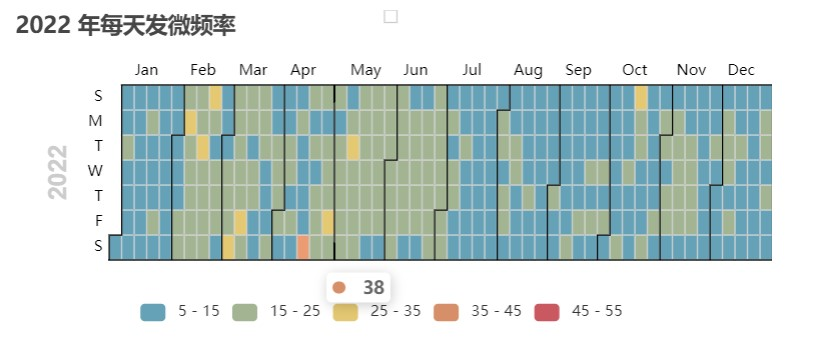
\includegraphics[width=12cm]{figure/2022.jpg}
    \caption{2022热力图} \label{fig:2022}
\end{figure}    
\begin{figure}[H]
    \centering
    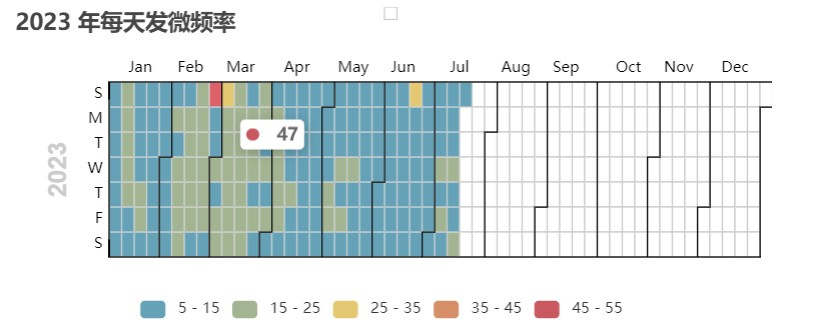
\includegraphics[width=12cm]{figure/2023.jpg}
    \caption{2023热力图} \label{fig:2023}
\end{figure}    

\subsection{发微时间统计}
使用pandas内置函数按照年、月、周、日、时分别统计共青团中央发微时间。
\begin{python}
    df = pd.read_csv('cleaned_text.csv', parse_dates=['created_at'])
    dateyear_counts = df['created_at'].dt.year.value_counts()
    datemonth_counts = df['created_at'].dt.month.value_counts()
    dateweek_counts = df['created_at'].dt.weekday.value_counts()
    dateday_counts = df['created_at'].dt.day.value_counts()
    datehour_counts = df['created_at'].dt.hour.value_counts()
\end{python}

\subsubsection{逐年统计}
利用pyecharts制作逐年统计可视化,结果如图\ref{fig:yearfre}所示。
\begin{python}
    c_year = (
        Bar()
        .add_xaxis([i[0] for i in resultyear])
        .add_yaxis("共青团中央", [i[1] for i in resultyear])
        .set_global_opts(
            title_opts=opts.TitleOpts(title="每年发微频率"),
            yaxis_opts=opts.AxisOpts(name="次数"),
            xaxis_opts=opts.AxisOpts(name="时间"),
        )

    )
\end{python}
\begin{figure}[H]
    \centering
    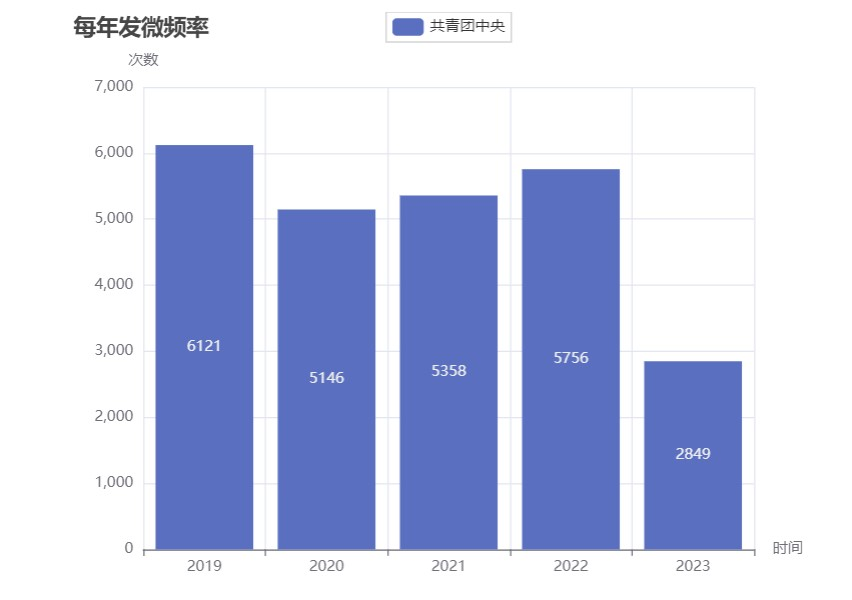
\includegraphics[width=12cm]{figure/yearfre.jpg}
    \caption{逐年统计} \label{fig:yearfre}
\end{figure} 
\subsubsection{每年逐月统计}
逐月统计可视化。
\begin{python}
    c_month = (
        Bar()
        .add_xaxis(Faker.months)
        .add_yaxis("共青团中央", [i[1] for i in resultmonth])
        .set_global_opts(
            title_opts=opts.TitleOpts(title="每月发微频率"),
            yaxis_opts=opts.AxisOpts(name="次数"),
            xaxis_opts=opts.AxisOpts(name="时间"),
        )

    )
\end{python}
\begin{figure}[H]
    \centering
    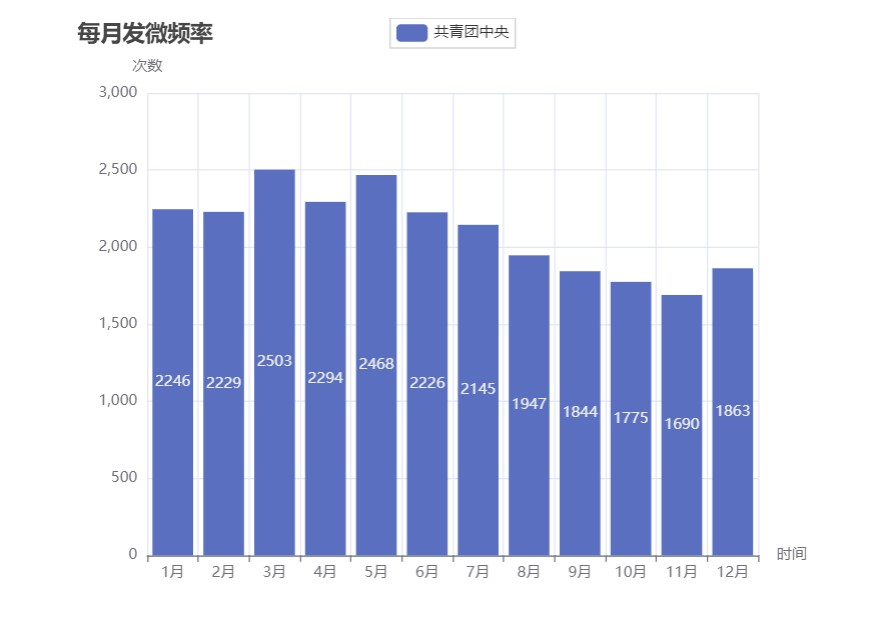
\includegraphics[width=12cm]{figure/monthfre.jpg}
    \caption{逐月统计} \label{fig:monthfre}
\end{figure} 
\subsubsection{每月逐天统计}
本小节后续部分与上述实现过程相似,不再赘述,仅展示最终可视化结果。
\begin{figure}[H]
    \centering
    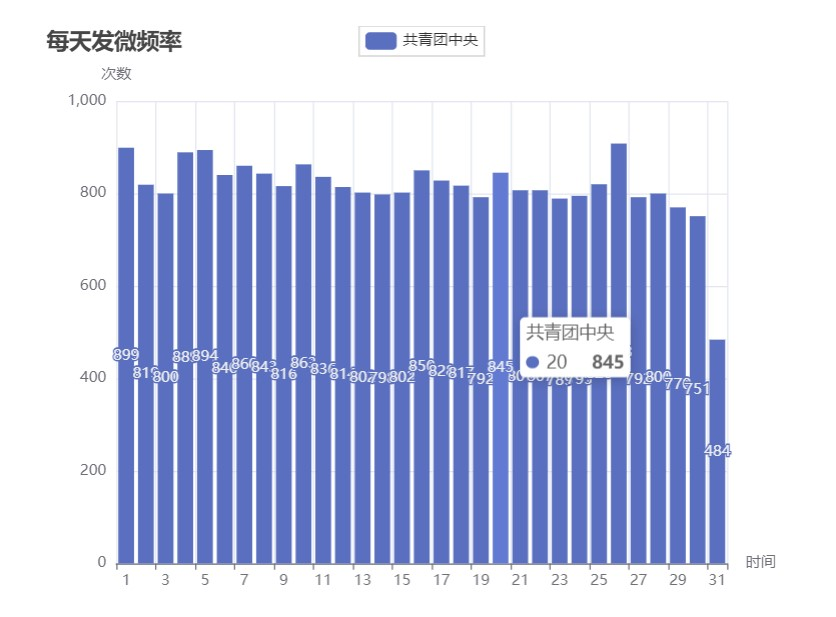
\includegraphics[width=12cm]{figure/dayfre.jpg}
    \caption{逐天统计} \label{fig:dayfre}
\end{figure} 
\subsubsection{每周逐天统计}
\begin{figure}[H]
    \centering
    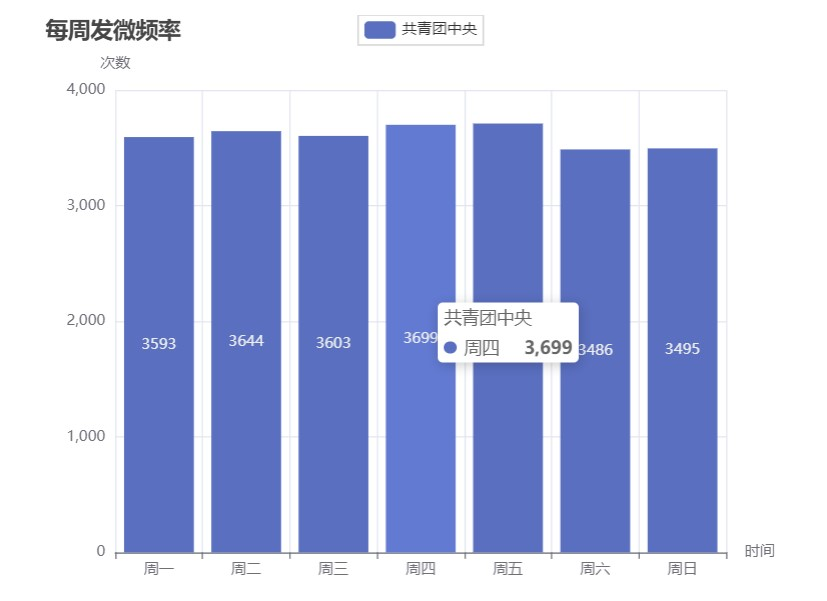
\includegraphics[width=12cm]{figure/weekdayfre.jpg}
    \caption{逐周统计} \label{fig:weekdayfre}
\end{figure} 
\subsubsection{每天逐时统计}
\begin{figure}[H]
    \centering
    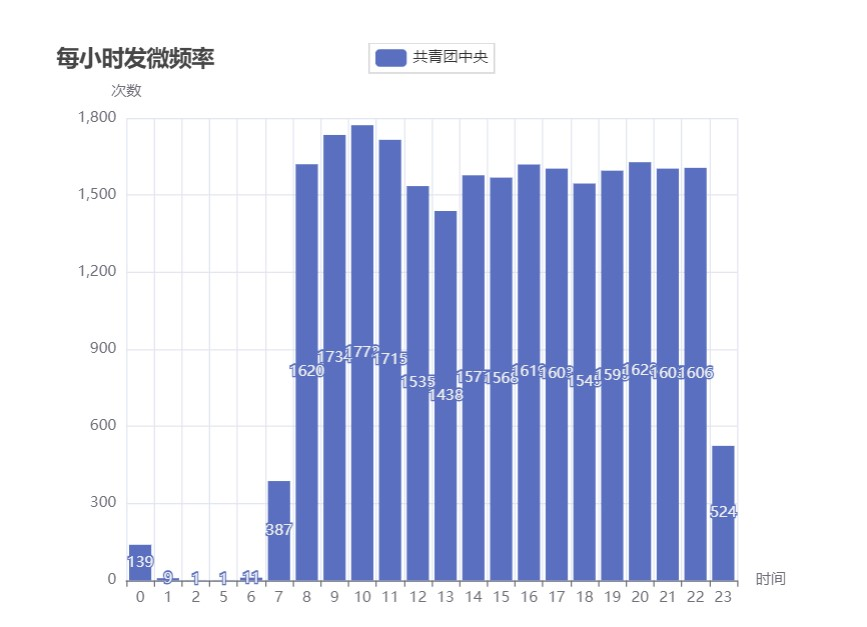
\includegraphics[width=12cm]{figure/hourfre.jpg}
    \caption{逐时统计} \label{fig:hourfre}
\end{figure} 
\subsection{周时热力统计}
\par{使用pandas的groupby多列分组先按照hour来分组。每组内,再按weekday来分组,并统计每个周时数量返回。}
\begin{python}
def to_weekhour(file, file_colm):
    df = pd.read_csv(file)
    df[file_colm] = pd.to_datetime(df[file_colm])
    hour_week_counts = df.groupby([df[file_colm].dt.hour, df[file_colm].dt.weekday])[file_colm].count()
    result = [[hour, week, count] for (hour, week), count in hour_week_counts.items()]
    result.sort(key=lambda x: x[0]) #按照第一个排序
    return result
\end{python}
\par{调用to\_weekhour函数将分类统计结果传回pyecharts进行可视化绘图,核心代码如下。}
\begin{python}
    c_heatmap = (
        HeatMap()
        .add_xaxis(Faker.clock)
        .add_yaxis(
            "发微次数", Faker.week, to_weekhour('cleaned_text.csv', 'created_at'),
            label_opts=opts.LabelOpts(position="middle")
        )
        .set_global_opts(
            title_opts=opts.TitleOpts(title="共青团中央发微周时热力图"),
            visualmap_opts=opts.VisualMapOpts(),
        )
    )
\end{python}
最终可视化效果如图\ref{fig:weekdayhour}
\begin{figure}[H]
    \begin{center}
    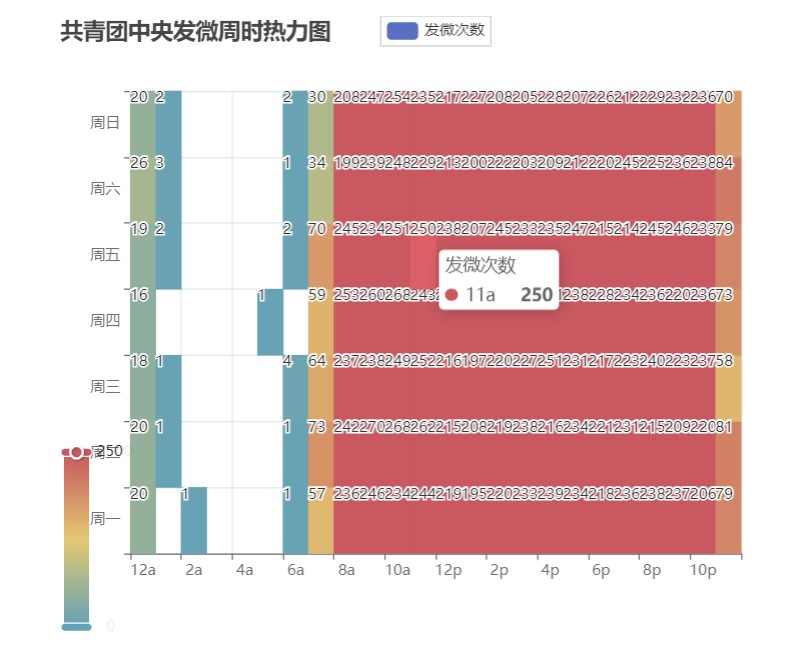
\includegraphics[width=14cm]{figure/weekday_hour.jpg}
    \caption{周时热力图}  \label{fig:weekdayhour}
    \end{center}
\end{figure}

\subsection{高频词统计}
定义函数统计词频,添加自定义词典和停用词词典,使用jieba库进行分词,jieba分词工具有三种主要分词模式,本报告选取\textbf{HMM}模式。
\begin{python}
def count_word_frequency(csv_file_path, column_name):
    df = pd.read_csv(csv_file_path)
    df[column_name].fillna('', inplace=True)
    content = df[column_name]
    merged_content = ' '.join(content)
    pattern = re.compile(u'\t|\n|\.|-|:|;|\)|\(|\?|"')
    string_data = re.sub(pattern, '', merged_content)
    jieba.suggest_freq('共青团', True)
    jieba.load_userdict('user_words.txt')
    seg_list_exact = jieba.cut(string_data, cut_all=False, HMM=True)  # 分词模式
    object_list = []
    # 去除停用词
    with open('stop_words.txt', 'r', encoding='UTF-8') as meaninglessFile:
        stopwords = set(meaninglessFile.read().split('\n'))
    stopwords.add(' ')
    for word in seg_list_exact:
        if word not in stopwords:
            object_list.append(word)
    word_counts = collections.Counter(object_list)
    for word in list(word_counts.keys()):
        if len(word) == 1:
            del word_counts[word]
    word_counts_top = word_counts.most_common(300)
    return word_counts_top
\end{python}
\par{使用pyecharts制作词云可视化,此外本报告也采用了自定义功能更强大的wordcloud库结合matplot等库制作了共青团中央微博内容词云可视化,相关结果为摘要页微博图标背景的词云可视化图片。}

\begin{python}
    c_wordcloud = (
        WordCloud()
        .add(
            "",
            count_word_frequency('cleaned_text.csv', 'content'),
            word_size_range=[20, 100],
            textstyle_opts=opts.TextStyleOpts(font_family="cursive"),
        )
        .set_global_opts(title_opts=opts.TitleOpts(title="top200词云"))
    )
\end{python}
使用pyecharts实现的可视化效果如图所示,能够实现在网页端点击悬停等交互。
\begin{figure}[H]
    \centering
    
\includegraphics[width=12cm]{figure/wordcloud_pyecharts.jpg}
    \caption{词频统计词云} \label{fig:wordcloud}
\end{figure} 

\subsection{LDA主题分析}
\par{首先对文本内容进行分词,分词程序位于analyze/LDA/cutword.py,具体实现与词云处一致调用jieba库。分词后,基于已分词文档使用gensim库进行LDA主题分析,并使用pyLDAvis进行可视化展示。思路阐述参考下列代码注释}\
\begin{python}
import pyLDAvis.gensim_models
from gensim.corpora.dictionary import Dictionary
from gensim.models.ldamodel import LdaModel
from gensim import corpora, models

if __name__ == '__main__':
    words_ls = []
    with open('outdemowei.txt', 'r', encoding='UTF-8') as f:
        data = f.readlines()
        for line in data:
            words_ls.append(line.split(' '))
    f.close()
    # 构造词典,将每个唯一的词语映射到一个唯一的整数ID
    dictionary = corpora.Dictionary(words_ls)
    # 基于词典,使【词】→【稀疏向量】,并将向量放入列表,形成【稀疏向量集】(即语料库)
    corpus = [dictionary.doc2bow(words) for words in words_ls]
    # tf-idf编码
    tfidf = models.TfidfModel(corpus)
    # 将语料库转换为tf-idf编码形式
    corpus_tf = tfidf[corpus]
    # lda模型,num_topics设置主题的个数
    lda = LdaModel(corpus=corpus_tf, id2word=dictionary, num_topics=4, random_state=100, iterations=50)

    for topic in lda.print_topics(num_words=10):
        print(topic)
    # 用pyLDAvis可视化
    plot = pyLDAvis.gensim_models.prepare(lda, corpus_tf, dictionary)
    pyLDAvis.save_html(plot, 'ldaweibo.html')

\end{python}
通过LDAModel抽取4个主题后,最终可视化效果如图\ref{fig:lda}所示,html可视化源文件位于analyze/LDA/ldaweibo.html。
\begin{figure}[H]
    \centering
    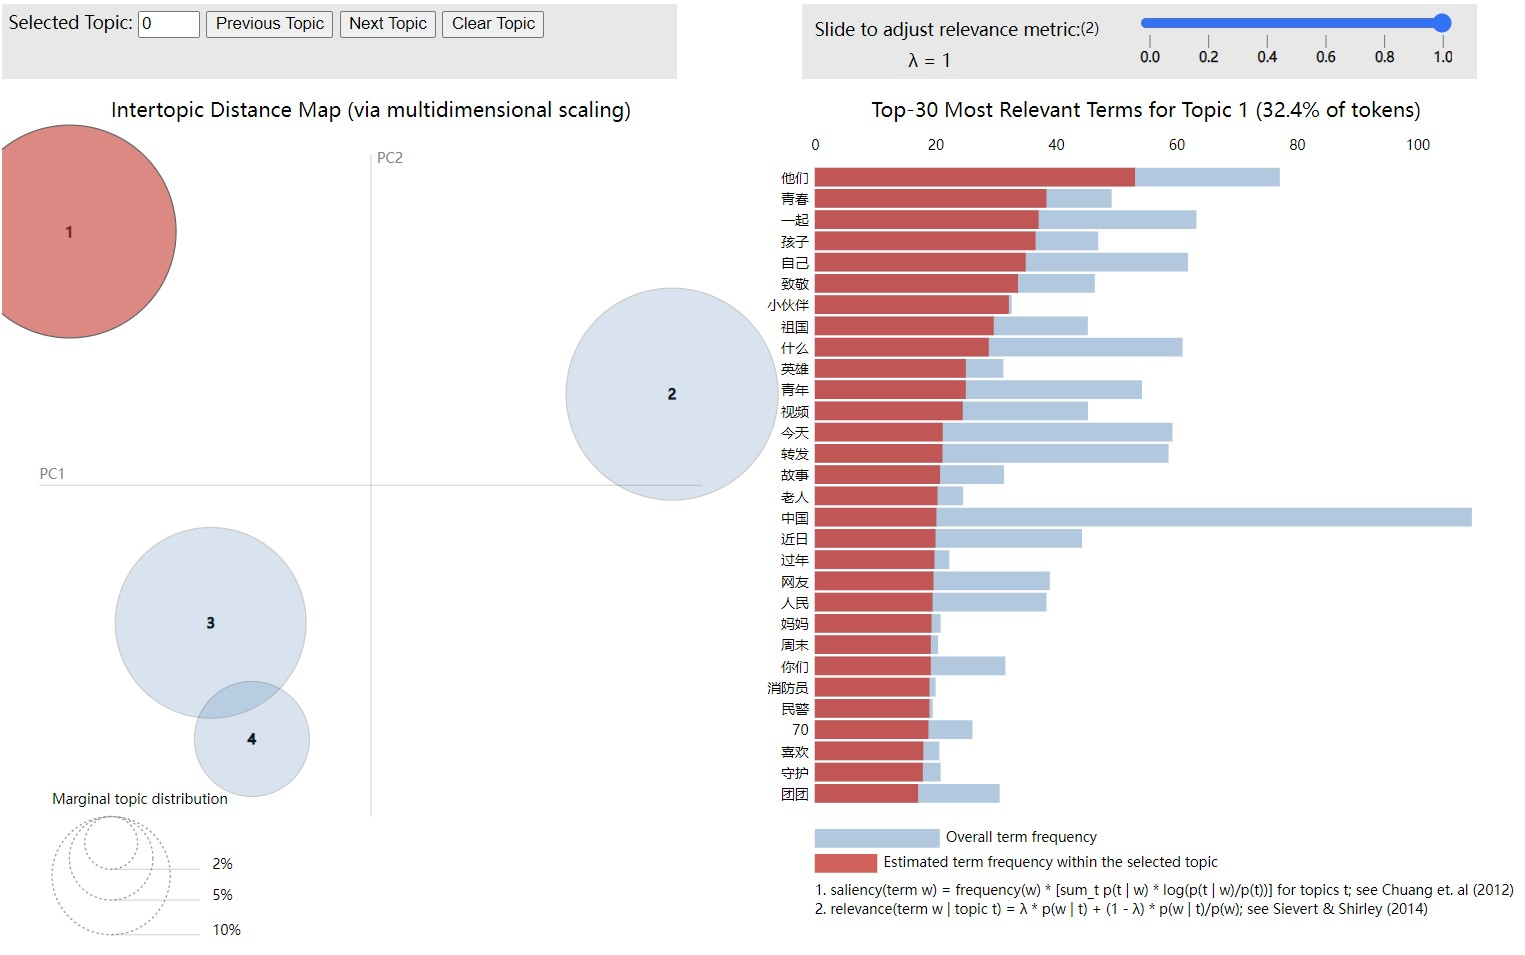
\includegraphics[width=12cm]{figure/lda.jpg}
    \caption{LDA分析结果} \label{fig:lda}
\end{figure} 

\section{总结展望}
\par{本文在python3.10环境下,基于对Github开源爬虫项目的改动实现数据爬取,调用了pandas,pyecharts,jieba,gensim等软件包,对所获得数据进行了统计分析和可视化交互展示。国内新闻传播顶刊有计算传播论文中写到利用python进行情感分析,使用snownlp进行分析,作为一个封装好的项目,再去调用已经没有难度,基础还是在于循环,判断等语句的应用。本报告并不试图去调用一些可能是用家具评论数据进行有监督机器学习的工具通过一行代码就能实现情感分析来用到自己所爬取的可能和模型预训练预料毫无关系的数据,试问这样的实现难度和简单写个函数让每一条数据调用分析后输出结果可视化有什么不同呢?背后更深的应该是整个模型实现的过程,有什么条件需要满足,能不能用到我的项目上。本报告也存在遗憾,在LDA分析的时候gensim库是做的无监督,但是确定主题数的时候没能实现一些暴力搜索之类的方法来确定主题数,还是人为尝试了很多数字之后确定的主题数,后续有时间一定解决这部分的遗憾实现编程的严谨。}
\par{写完报告主体想到读过的很多新闻传播论文,真诚希望很多文章在使用某个方法非要去赋予概念的时候能够多一点技术理性,首先理解技术逻辑、判断自己的项目是否适合使用该数据分析技术、最终分析社会问题,否则如果仅仅是冠以计算和智能的tag毫无判断也无法读懂方法核心为了让自己的研究显得更“高端”、方法更新,在用一个错误的手段分析社会解读社会,这个世界真的会因为所谓学术更好嘛?}
\par{老师对待计算机,对待编程,对待技术、对待社会的严谨,从中收获很多。希望国内计算传播越来越好!}


%============= 参考文献 =====================
%\addcontentsline{toc}{section}{参考文献}
%\bibliography{bibfile}
\clearpage
%=============  致谢  ======================
%\section*{致谢}
\addcontentsline{toc}{section}{致谢}
谢谢!!!
%\newpage
\appendix
\section代码与注释}

\begin{python}
def 

\end{python}


\end{document}
%%%%%%%%%% 结束 %%%%%%%%%%